\documentclass[a4paper,10pt]{article}
%\usepackage[utf8x]{inputenc}

\usepackage{graphicx}
\usepackage{float}
\usepackage{caption}
\usepackage{subcaption}
\usepackage{amsmath}


%opening
\title{Assignment 4: Optical Flow and Structure from Motion}
\author{Robrecht Jurriaans (5887380), Taco Cohen (6394590)}

\begin{document}

\maketitle

\section{Optical Flow}

We have implemented Lucas-Kanade optical flow for a single scale on both synthetic images and on a sequence of a model house. For the synthetic images, optical flow was computed on a grid of non-overlapping $15\times15$ windows, whilst a set of points was tracked over the model house sequence. We created two separate functions for this: \verb|LucasKanade.m| for the non-overlapping windows and \verb|LK_M.m| for the tracking. 

\begin{figure}[h!tb]

        \centering
        \begin{subfigure}{0.475\textwidth}
                \centering
                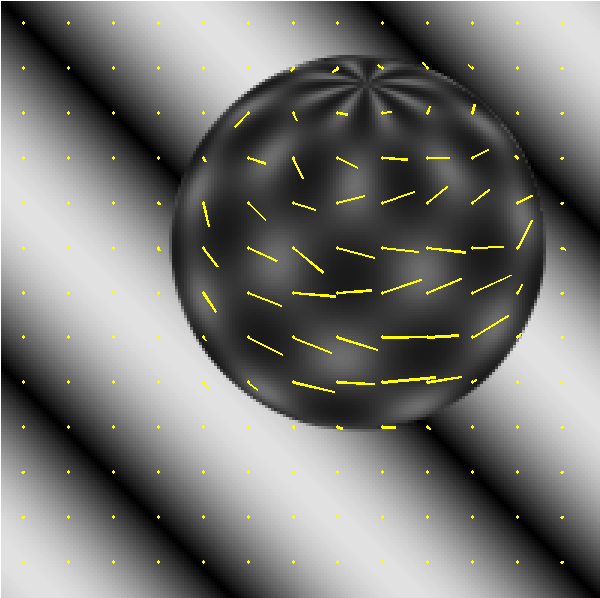
\includegraphics[width=\textwidth]{sphere}
                \caption{Optical flow for the sphere images}
        \end{subfigure}
        ~
        \begin{subfigure}{0.475\textwidth}
                \centering
                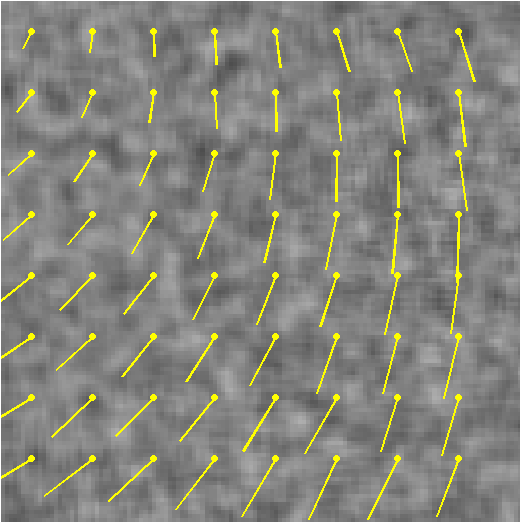
\includegraphics[width=\textwidth]{synth}
                \caption{Optical flow for the synth images}
        \end{subfigure}
\caption{Optical flow for non overlapping $15\times15$ windows, circle denotes origin of optical flow vector}
\label{fig:opflow}      
\end{figure}

\subsection{Sphere and Synthetic Images}
In figure \ref{fig:opflow} the resultant optical flow vectors can be seen for both the \emph{sphere} images as the \emph{synth} images. The sphere is turning to the right, which can be seen in the optical flow vectors on the sphere. Some of the flow vectors seem to be a bit off, but this is mainly because the windows were not centred at good features which would improve results. The synthetic image rotates slightly around the top left corner and this result can be seen in the right image.



\subsection{Optical flow on the model house sequence}
The model house sequence consist of 101 frames with 215 given points which can be tracked. In figure \ref{fig:modelhouse} the 100th frame can be seen with the ground truth and the corresponding points as tracked by the algorithm. The final sum of squared errors is $337.3183$ and the median squared error is $17.3528$. The main contributor to the error are points which drift into ``flat'' regions in which no motion can be observed causing the points to further drift away from the ground truth. Another contributor is the \emph{jpg} compression of the sequence, causing noise in the data which result in less precise optical flow vectors.

\begin{figure}[h!tb]
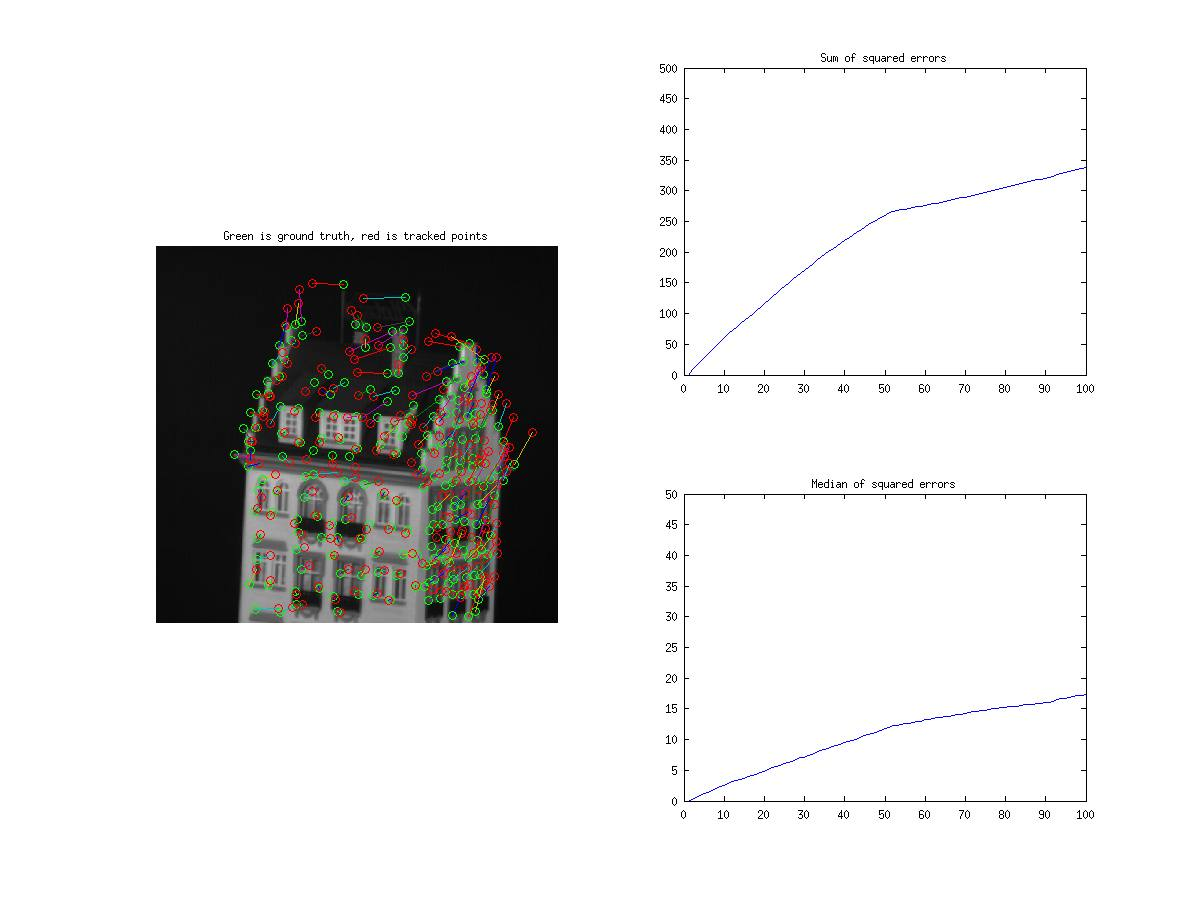
\includegraphics[width=1\textwidth]{frame00000100}
\caption{Frame 100 from the model house sequence, green circles represent ground truth, red circles are the points tracked over all 100 frames, lines connect corresponding points, the graphs represent the sum of squared errors and the median of squared errors over the sequence }
\label{fig:modelhouse}
\end{figure}

A movie was created of the output frames: \verb|opflow.avi| in which this effect can be clearly seen. This is especially the case for the points on the left of the house which drift into the dark background.

\clearpage

\section{Structure from Motion}

We implemented Structure from Motion (SfM) by the Tomasi-Kanade Factorization method.
We first generate a measurement matrix $D$, either by reading the ground truth from disk or using the outputs of our Lucas-Kanade point tracker.
This matrix has the image $(x,y)$ coordinates of point $j$ in view $i$ at $D_{2*i, j}$ and $D_{2*i+1,j}$.
We construct the Shape matrix $S$ and Motion matrix $M$ by using SVD on this matrix (distributing diagonal matrix $W$ equally among the two).

The points can be plotted now (they are simply the columns of $S$), but the resulting figure is affinely skewed from the ground truth, see figure \ref{fig:affine}.
The reason is that we have so far only imposed affine constriants.
To retrieve the true structure, we further impose Euclidean constraints as follows.

We can split $M$ into chunks $A_i$, that multiply each 3D point to produce its 2D projection on image $i$.
The rows of this matrix correspond to the image axes, which we will constrain to be of unit-length and orthogonal to each other:
$a_1^T a_2 = 0$, $a_1^T a_1 = 1$ and $a_2^T a_2 = 1$.
If we transform these by a matrix $Q$, we get the transformed constraint $(Q a_1)^T (Q a_2) = a_1^T (Q^T Q) a_2 = 0$, and similarly for the others.

Let $L$ be the symmetric matrix $L = Q Q^T$, then we have three linear equations in $L$ for each camera.
We could write this out, but it is a big $3 \times 6$ matrix with entries that are quadratic in $a_i$.
So instead we refer the reader to \verb+TomasiKanadeFactorization.m+, where this is implemented.

We stack each of these equations in a large $3m \times 6$ matrix (3 equations for each camera, 6 unknowns in a $3\times 3$ symmetric matrix), and solve for the parameters of $L$ using least-squares.
We then factorize $L = Q Q^T$ using Cholesky decomposition, and update $M = M Q$ and $S = Q^{-1} S$.
The result is show in figure \ref{fig:Euclidean}.

Finally, we applied the Tomas-Kanade algorithm to the output of the Lucas-Kanade algorithm.
The results are a bit more noisy, as can be seen in figure \ref{fig:kamikaze}.

The code can be tested by running  \verb+SFMdemo.m+, which plots Affine structure from ground-truth, Euclidean structure from ground-truth, Affine structure from LK tracker, and Euclidean structure from LK tracker.
When viewing results, please select the rotation tool, then right-click and select Rotate Options/Fixed Aspect Ratio.

\begin{figure}[h!tb]

        \centering
        \begin{subfigure}{0.3\textwidth}
                \centering
                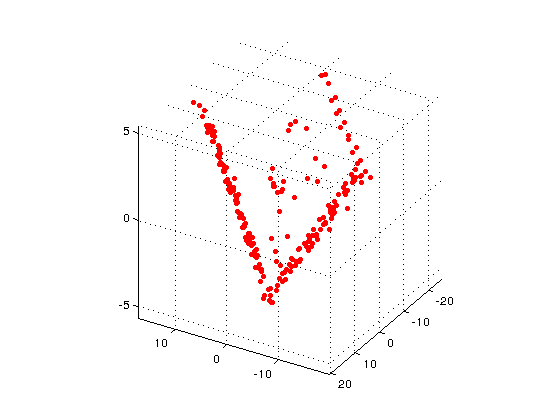
\includegraphics[width=\textwidth]{AffineStructure1}
                \caption{View 1}
        \end{subfigure}
        ~
        \begin{subfigure}{0.3\textwidth}
                \centering
                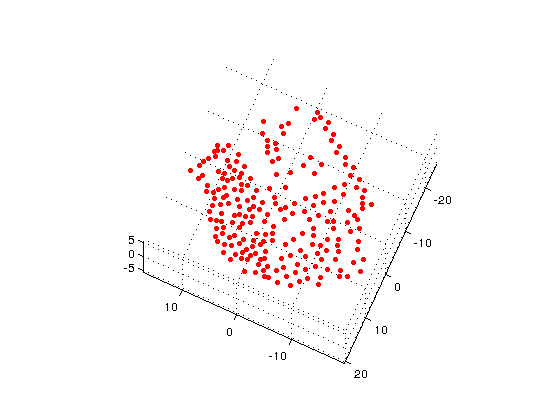
\includegraphics[width=\textwidth]{AffineStructure2}
                \caption{View 2}
        \end{subfigure}
        ~
        \begin{subfigure}{0.3\textwidth}
                \centering
                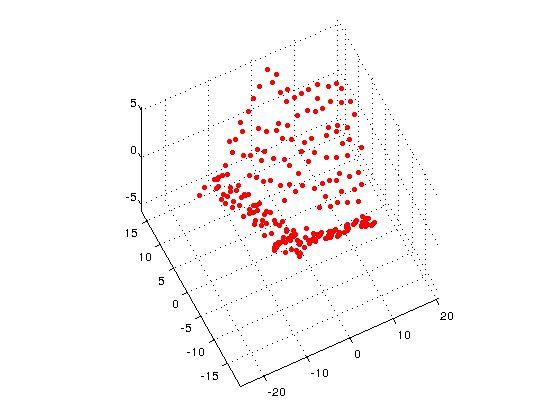
\includegraphics[width=\textwidth]{AffineStructure3}
                \caption{View 3}
        \end{subfigure}
\caption{Affine structure from motion (using groud-truth points as input). Notice the affine skew, which is particularly obvious in view 1.}
\label{fig:affine}      
\end{figure}

\begin{figure}[h!tb]

        \centering
        \begin{subfigure}{0.3\textwidth}
                \centering
                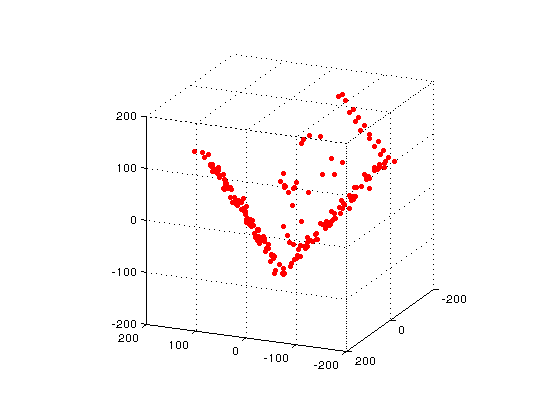
\includegraphics[width=\textwidth]{EuclideanStructure1}
                \caption{View 1}
        \end{subfigure}
        ~
        \begin{subfigure}{0.3\textwidth}
                \centering
                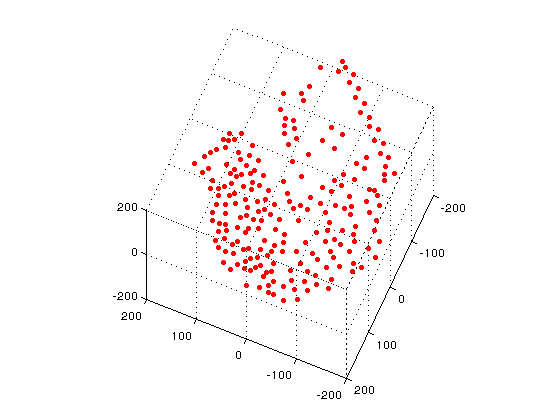
\includegraphics[width=\textwidth]{EuclideanStructure2}
                \caption{View 2}
        \end{subfigure}
        ~
        \begin{subfigure}{0.3\textwidth}
                \centering
                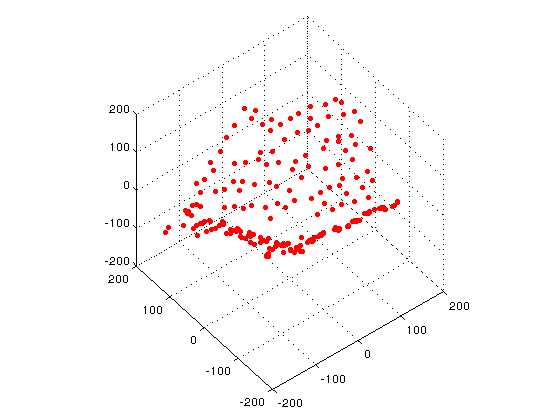
\includegraphics[width=\textwidth]{EuclideanStructure3}
                \caption{View 3}
        \end{subfigure}
\caption{Euclidean structure from motion (using ground-truth points as input). Notice that the true Euclidean structure has been recovered: the walls are now orthogonal.}
\label{fig:Euclidean}      
\end{figure}


\begin{figure}[h!tb]

        \centering
        \begin{subfigure}{0.3\textwidth}
                \centering
                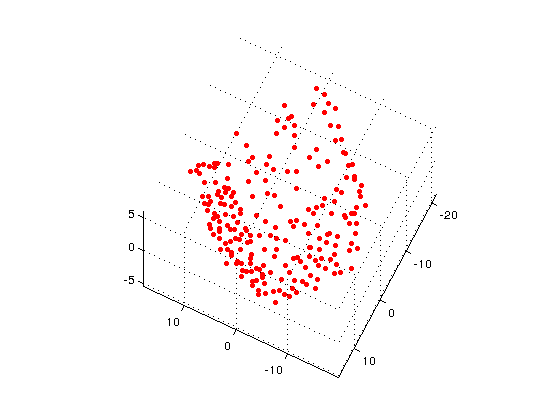
\includegraphics[width=\textwidth]{AffineStructureLK}
                \caption{Affine}
        \end{subfigure}
        ~
        \begin{subfigure}{0.3\textwidth}
                \centering
                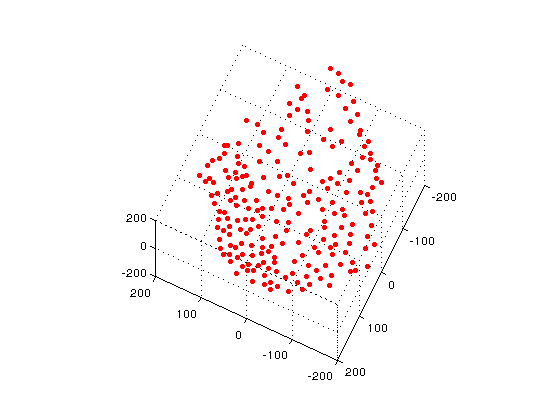
\includegraphics[width=\textwidth]{EuclideanStructureLK}
                \caption{Euclidean}
        \end{subfigure}

\caption{Affine and Euclidean structure from motion, using the result of the LK tracker as input.}
\label{fig:kamikaze}      
\end{figure}


\end{document}
